\section{Numerical Experiments}

To show accuracy and efficiency, we designed two numerical experiments for the adaptive rebuild algorithm for the \gls{qahps} method. The first is a uniform refinement and coarsening starting from an initial mesh to show convergence. In the second, an initial mesh is randomly refined multiple times and we observe the time 

\subsection{Refinement/Coarsening Convergence Test}
\label{sub:refinement-coarsening-test}

We solve a Poisson equation
\begin{align}
    \nabla^2 u(x, y) = -(\sin(x) + \sin(y))
\end{align}
subject to Dirichlet boundary conditions. We start with an initial mesh refined uniformly to $L_{\text{min}} = 1$ with $M = 16$. There are two parts to this numerical experiment.

{\bf Part One: Refinement} 
First, we compute the initial factorization and solution by calling the build, upwards, and solve stages. Next, we refine the mesh to $L_{\text{min}} + 1$, then to $L_{\text{min}} + 2$, and so on until $L_{\text{min}} = L_{\text{max}}$. Computing the solution is done in two ways: via the {\em full build} where the build, upwards, and solve stages are called, and via the {\em adaptive build} where the factorization is adapted from the initial mesh. This is done according to the adaptive rebuild algorithm from \refsec{sec:adaptive-rebuild-algorithm} (by just calling the upwards and solve stages). After each refinement, we compute and report the error.

{\bf Part Two: Coarsening}
After refining the mesh to $L_{\text{max}}$, we successively coarsen the mesh level by level until we arrive back at $L_{\text{min}}$. After each coarsening, we compute and report the error of the full build and the adaptive build.

{\bf Discussion}
The results of this numerical experiment can be found in \reffig{fig:full-vs-adaptive-convergence}. The left plot shows the convergence starting from $L_{\text{min}}$ up to $L_{\text{max}}$, while the right plot shows the convergence from $L_{\text{max}}$ to $L_{\text{min}}$. We should expect that the two methods obtain the exact same solution as both methods use the same merge and split algorithms. This test verifies this claim.

Additionally, we can note that this method maintains the $2^{nd}$ order accuracy as prescribed in this implementation of the \gls{qahps}. When initializing new patches, we use a $2^{nd}$ order accurate bilinear interpolation scheme to move from coarse patches to refined patches and vice versa.

\begin{figure}
    \centering
    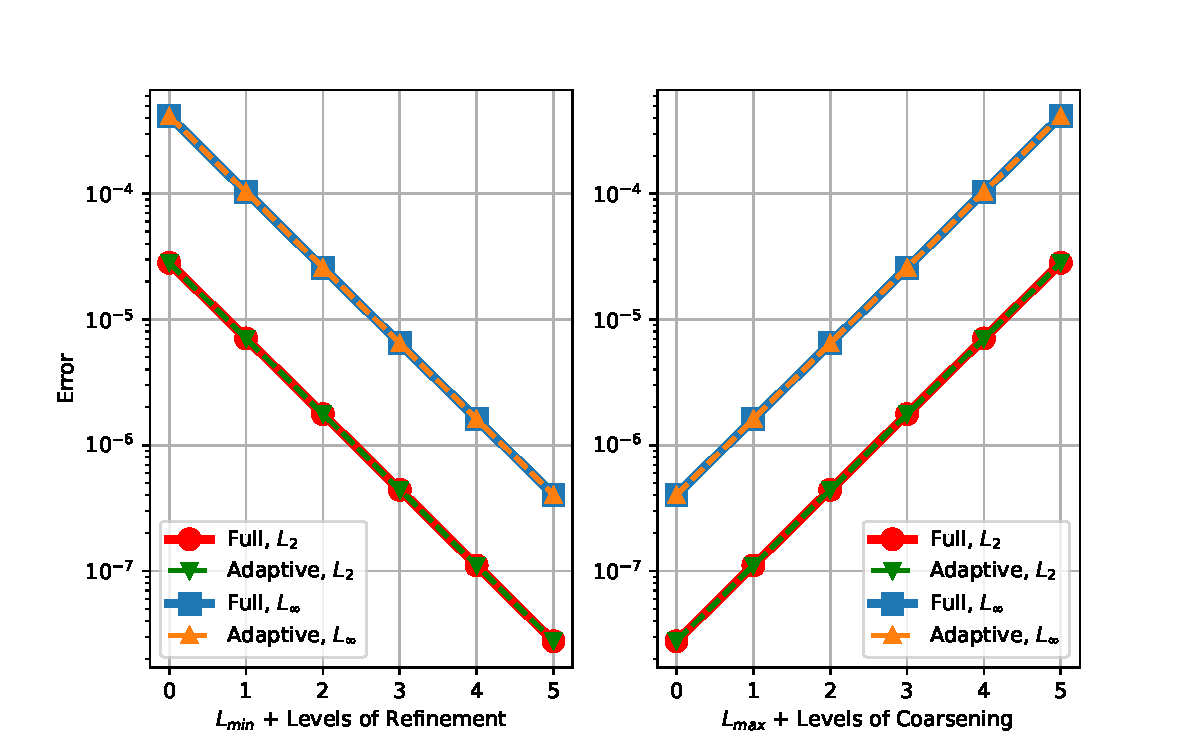
\includegraphics[width=\textwidth, clip=true, trim={20 0 40 40}]{figures/full-vs-adaptive-convergence-no-title.pdf}
    \caption{Convergence test for the adaptive rebuild algorithm (\refsec{sec:adaptive-rebuild-algorithm}). Both plots show the full build and the adaptive build methods used to solve a Poisson problem. The left plot shows the convergence starting from $L_{\text{min}}$ up to $L_{\text{max}}$, while the right plot shows the convergence from $L_{\text{max}}$ to $L_{\text{min}}$.}
    \label{fig:full-vs-adaptive-convergence}
\end{figure}

\subsection{Random Refinement}
\label{sub:random-refinement}

In this numerical experiment, we seek to compare the timing between a full build and an adaptive build when solving successive elliptic \gls{pdes}. We start with an initial uniform mesh refined to $L = 5$ with $M = 16$. The initial factorization and solution are computed on this mesh. Then, we pick a random leaf patch and tag it for refinement. After refinement, the solution on the new mesh is computed using either the full \gls{qahps} method, or the adaptive-rebuild version as outlined in this chapter. The random nodes are cataloged to ensure that both methods are solving on the same mesh. For each solve, we report the time to refine the mesh, as well as the build, upwards, and solve stages of the \gls{qahps} method.

{\bf Discussion}
As shown in \reffig{fig:full-vs-adaptive-time-comparison}, the time to solution for each successive solve is much faster for the adaptive-rebuild method. For the full \gls{qahps} method, the build stage dominates the time per iteration. The build stage can effectively be done only once per level instead of for all families in the quadtree. Updating the factorization set $\mathcal{S}$ during the refinement does add overhead to the refinement process (and would do so for coarsening as well), however, this overhead is minimal compared to the full merge traversal for the build stage. The timing for the upwards and solve stages for both methods remains the same, which is expected.

\begin{figure}
    \centering
    \begin{subfigure}[t]{1\textwidth}
        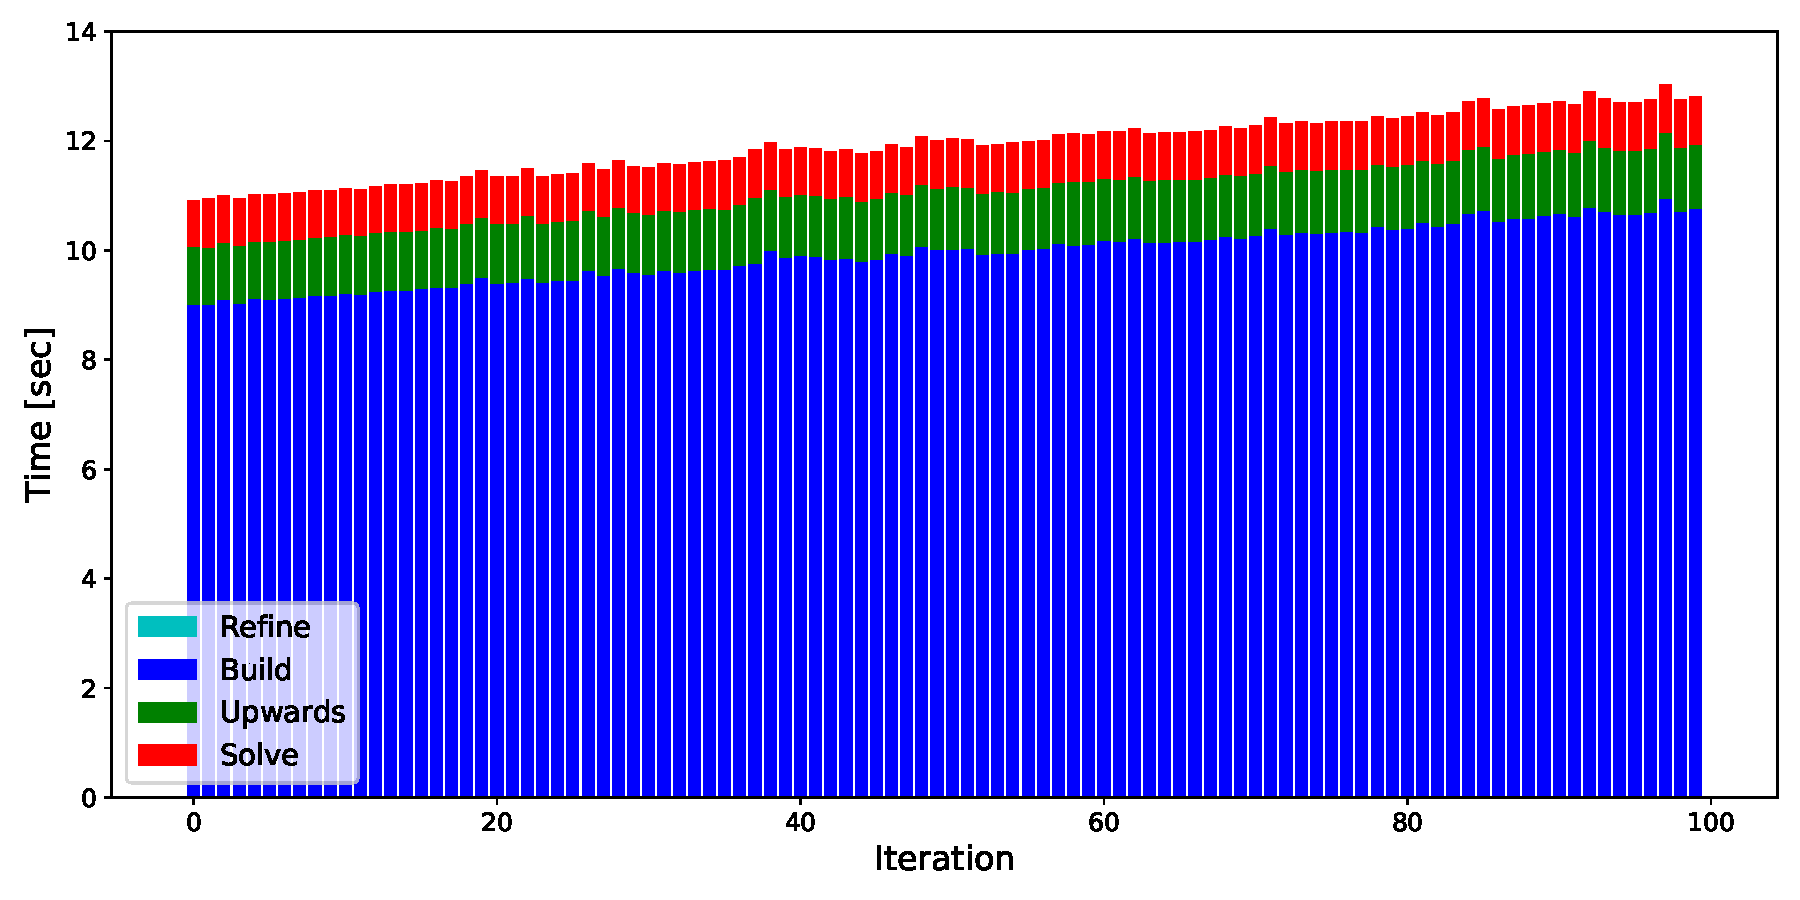
\includegraphics[width=\textwidth, clip=true, trim={10 10 10 10}]{figures/full-stacked-bar-no-title.pdf}
        \caption{Full build method}
        \label{fig:full-time-comparison}
    \end{subfigure}
    \begin{subfigure}[t]{1\textwidth}
        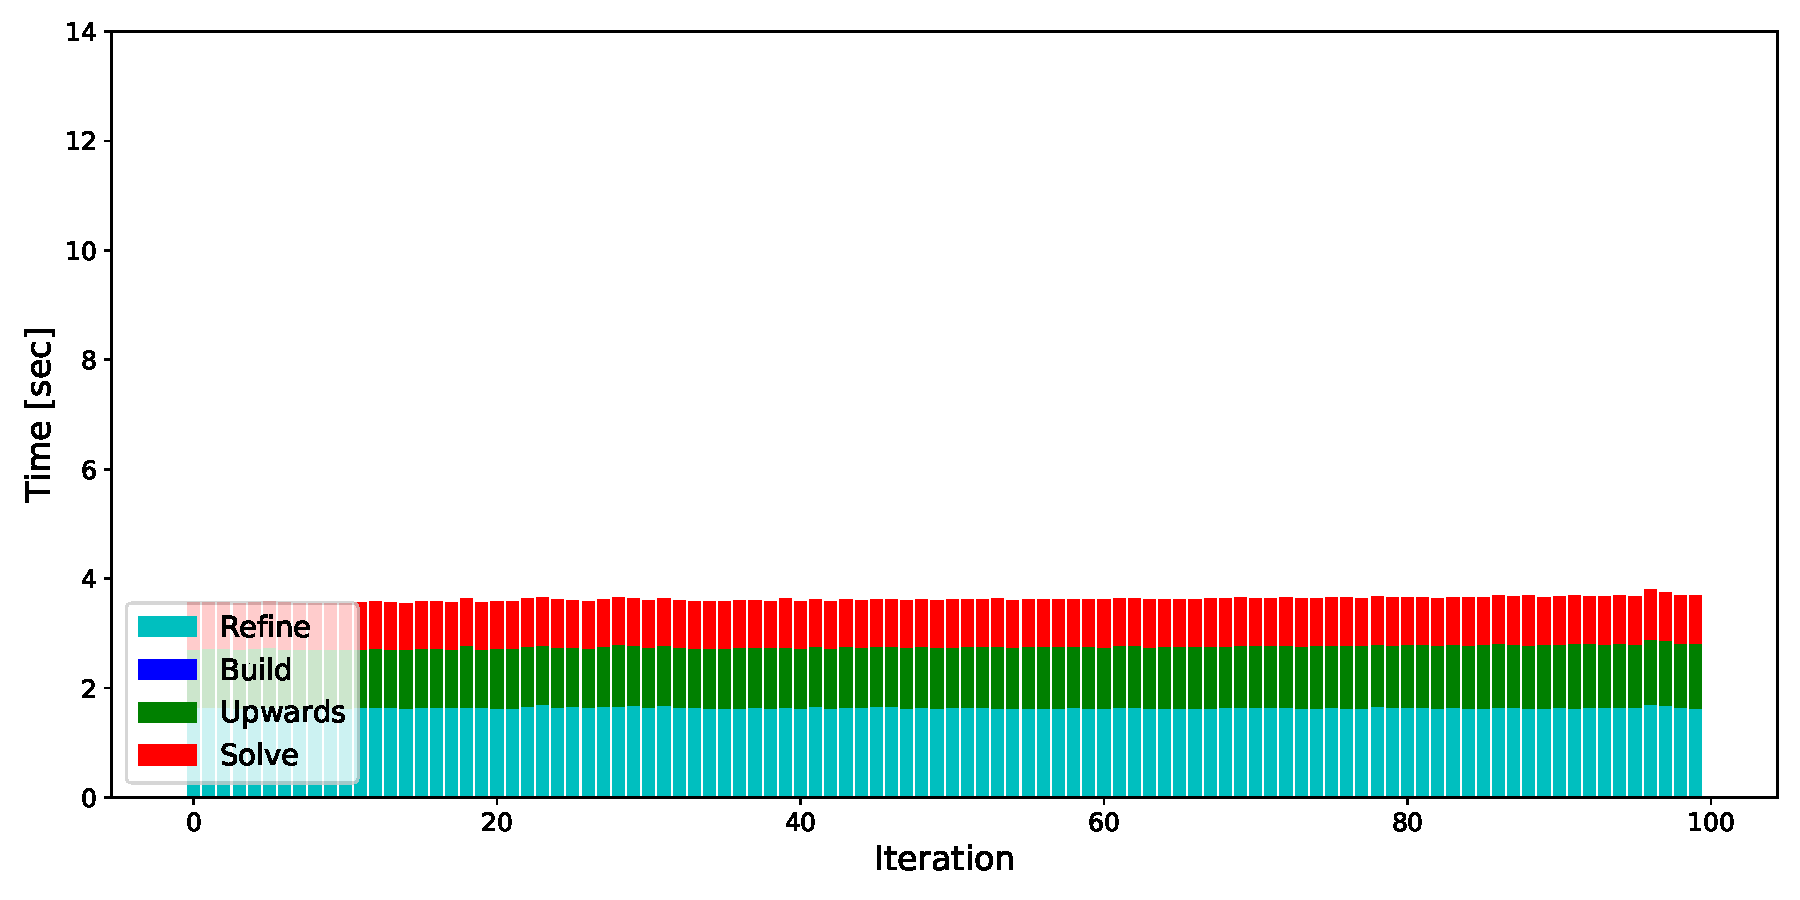
\includegraphics[width=\textwidth, clip=true, trim={10 10 10 10}]{figures/adaptive-stacked-bar-no-title.pdf}
        \caption{Adaptive build method}
        \label{fig:adaptive-time-comparison}
    \end{subfigure}
    \caption{Comparison of full vs. adaptive build methods for the random refinement experiment (\refsec{sub:random-refinement}). In each iteration, a random leaf node is refined and the elliptic problem is solved with the QAHPS method. Lower is better.}
    \label{fig:full-vs-adaptive-time-comparison}
\end{figure}